% \chapter{Arquitectura y comandos b\'asicos}
\chapter{Introducci\'on a Grails}
\section{Arquitectura}
Grails envuelve a muchas tecnolog\'ias relacionados con \textit{java}, abstrayendo su complejidad al proporcionarnos configuraciones predeterminadas que cubren los casos de uso m\'as comunes. Estas configuraciones pueden ahorrarnos d\'ias o semanas de trabajo debido a la integraci\'on con otras tecnolog\'ias.

Aqu\'i se presentan las tecnolog\'ias principales sobre las que se Grails est\'a montado:
%En este cap\'itulo se listan las tecnolog\'ias que usa grails y comandos b\'asicos para comenzar a usarlo. 

\begin{multicols}{2}
\begin{itemize}
  \item Hibernate
  \item Spring
  \item Sitemesh
  \item Tomcat
  \item H2
  \item Groovy
  \item Gant
  \item JEE
\end{itemize}
\end{multicols}

\begin{figure}[ht!]

    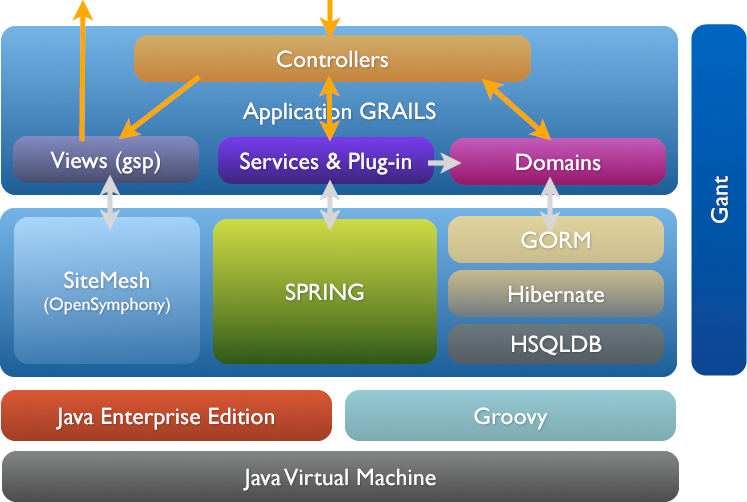
\includegraphics[width=100mm]{img/arch}
    \caption{Tecnolog\'ias que confirman la arquitectura de Grails}
    \label{arquitectura}

\end{figure}


\newpage
\section{Artefactos de Grails}
Grails consta de cuatro tipos de artefactos principales:
\begin{enumerate}
 \item Views
 \item Controllers
 \item Domains
 \item Services
\end{enumerate}

\subsection{Views}
Muestran informaci\'on al usuario de la aplicaci\'on. En Grails, las vistas existen en forma de archivos con extensi\'on \textit{gsp}. La informaci\'on es puesta en los \textit{gsp} a trav\'es de plantillas\footnote{Para los m\'as experimentados, llenar estas plantillas usan una sintaxis intermedia entre tags \textit{jstl} y tags de \textit{jsf}} y estas se llenan a trav\'es de controllers. 

\subsection{Controllers}
Se encargan 
\subsection{Dominios}
\subsection{Servicios}